\chapter{Evaluation}\label{Chap:Evaluation}

Having developed the PARRHI system it is now time to ask, whether or not the end goal was actually achieved. For that, I will shortly summarize the requirements collected in section~\ref{Section:Requirements}. The Developer (the person that uses the PARRHI system to create applications) has no to little software engineering skills but some knowledge about the robot industry. The person would like to reuse their previous work and create Augmented Reality Applications for other people to use. The application should transfer some knowledge, or give instructions on how to achieve a certain task.

This evaluation will consist of two different parts. First I will try to compare traditional AR programming methods with the PARRHI system, and then I will let other people try to succeed in a specific task that was given to them. 

\section{Evaluation 1: Comparing PARRHI with traditional methods}

I will first define a use case for the evaluation, then pose as the "Developer" and actually develop such a AR application. First, it will be manually programmed without the PARRHI system. For future reference, this run will be called the "\textit{manual attempt}". Then, I will attempt to achieve the same goal by using the PARRHI system. This run will be called the "\textit{PARRHI attempt}". Both attempts will be timed and afterwards I will compare the Pros and Cons of each approach.

\subsection{Evaluation 1: Use Case Definition}
The following use case will be the base of my thesis' evaluation. As a context, I will use the same factory as explained in section~\ref{Section:UseCaseDefinition}. 

The task, which will be supported by an Augmented Reality Robot Human Interface is the following. First, the employee using the AR application approaches the robot work cell and will then be commanded to walk over to a specific point, that is in a safe distance from the robot. After that, the person has to move the robot's TCP close to his position, so that they can touch the robot's tip. The user will be asked to remove the item in the robot's gripper and jog the robot back into its starting position. Having reached this position, the user will be told to move away into a marked area. The robot will then drive into his "zero" position, where all joint angles are 0 degrees. 

This task involves multiple objects in the robot factory, including the robot itself, the user's position, jogging the robot and walking round. To keep the scope of this evaluation at a reasonable level, I will allow myself to reuse the Robot-Library and the image recognition parts for the \textit{Manual attempt}. 

\subsection{Evaluation Manual Attempt}

The manual attempt is defined by programming the task described above manually. I used the same programming language and game engine as I did during the development of the PARRHI system, which means, that I could reuse the complete project setup including libraries and tools. It took about 2.5 hours to develop a reasonably good framework that allows for an easy implementation of the task. For that, I reused the Robot forward kinematics model and the robot library that handles the communication between any .NET Framework application and the robot controller. 

The implementation of the actual task for the AR application took about 1 hour. I implemented the steps relatively minimalistic, meaning, that I did not invest a lot of work and time into the styling of holograms and kept it at a basic level in general.

I will now summarize the downsides and benefits of the manual attempt, where unfortunately, the developer absolutely must be an experienced programmer, know the basics of forward kinematics, Unity, $C\#$ development, AR, Image tracking and more. Although the most complicated tasks like image tracking are done by some third party libraries, the developer has to know how to use them effectively. Also the Unity Engine is not perfectly intuitive, and might need some training time, to get up to speed.

The upside of course is, that any non-trivial task can be achieved. If one step in the application involves complex logic or simply some actions that are not supported by the PARRHI system, the developer can simply add the feature on the fly, because they are developing everything in source code anyway. The downside of this is, that also the most trivial processes have to be worked out in source code every time they occur. Furthermore, developing the application in Unity itself means, that the product has to be compiled, built and then transferred to the HoloLens every single time something changes. This process takes about 3-5 minutes and is very error prone.

Depending on the project's architecture, one could get into trouble if some task requirements change. Reusing the accomplished work is possible, but it involves a number of steps, where each and every one can cause errors. In order to go into more detail here, I would have to explain how Unity works, which is not within the scope of this thesis. 

\subsection{Evaluation PARRHI Attempt}
The PARRHI attempt means, that the same use case as above was be implemented using the PARRHI system. Based on the default template of the Parametrised Program, which contains the basic XML structure and defines the needed objects to animate the robot, it took about 15 minutes to complete the given task. It is important to mention, that I know the PARRHI syntax very well and did not need any time to get used to it. But, the same is true for the manual attempt with Unity.

The Parametrised Program for this task contains four point definitions, eight triggers for the individual steps and 21 actions that are executed by the triggers. This use case was easily achievable with the PARRHI system, because all needed actions are supported. 

The structure is very easy. There are eight steps that represent eight individual phases in the task. Each step has one trigger, that marks its end and invokes the needed actions to transition into the next step. 

\subsection{Conclusion Evaluation 1}
Comparing the two methods described above, I come to the conclusion, that using the PARRHI system definitely speeds up the development process but at the same time might limit the developer's possibilities. 

For trivial tasks, the PARRHI system greatly speeds up and simplifies the development process of these applications. A potential developer needs much less time to get used to the programming environment, than it would be the case with traditional programming and most importantly does not have to be a software engineer to do so. The developer can invest more time into the applications workflow using their domain-specific knowledge, when using the PARRHI system, since all AR and many other aspects are done by the PARRHI system.

But PARRHI's strengths are its biggest weaknesses. As soon as a developer needs a feature that is not supported by the PARRHI system, other solutions have to be found. There is currently no way of extending the trigger/action system with custom objects. This is due to the big simplification that had to be undertaken in the concept of the Parametrised Program, so that non software engineers are able to develop Augmented Reality Robot Human Interfaces. 

This limitation really only applies to specific features that are not supported by actions or triggers. The PARRHI system is indeed capable of creating high complexity workflows.. Parallelisation for example is not a problem in the PARRHI system. It would be perfectly fine to have two workflow branches running at the same time. 

A solution to the mentioned weaknesses discovered in this evaluation will be proposed in section~\ref{Section:FutureWork}.

\section{Evaluation 2: New Developers}
As shorty described in this chapter's introduction, the second evaluation will test the systems usability by letting other people try to achieve a certain task. First, I will again define a Use Case for them to achieve and then summarise their findings and feedback.

\subsection{Evaluation 2: Use Case Definition}
The task for the experimentees will be to create an AR HR Interface with the Parametrised Program that helps the User to do the following task:

\FloatBarrier

\begin{figure}[!h]
	\begin{minipage}{0.4\textwidth}
		\centering
		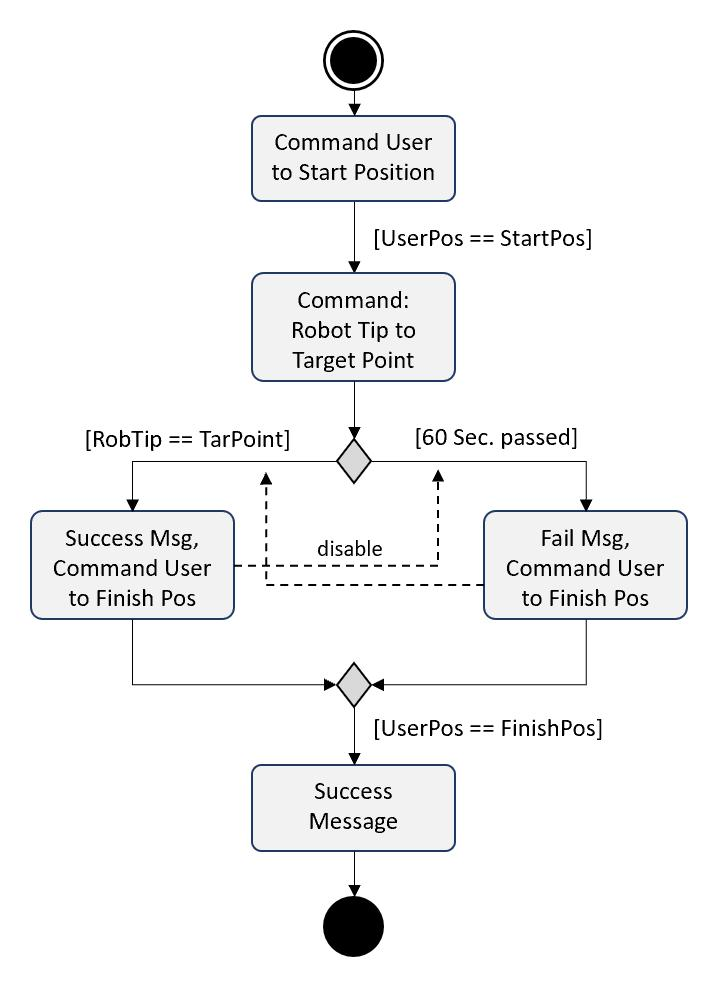
\includegraphics[width=1\linewidth]{Figures/Evaluation2_workflow}
		\caption[Evaluation 2 UseCase Workflow]{}
		\label{Fig:Evaluation2Workflow}
	\end{minipage}\hfill
	\begin{minipage}{0.55\textwidth}
		\begin{enumerate}
			\item The User should approach the robot safely by walking to the Start Position.
			\item Then, the robot should be jogged into a given position in under 1 minute.
			\item The application should then display a success or failure message according to step 2.
			\item In both cases, the user should be commanded to move away into the finishing position, such that the robot can not inflict any damage.
		\end{enumerate} 
		The coordinates of the Start, Finish and Robot-Target Points will be given to the experimentees. Fig.~\ref{Fig:Evaluation2Workflow} depicts one solution to the given task as a workflow diagram. 
	\end{minipage}
\end{figure}

\FloatBarrier

Each experimentee will be given a 15 minute explanation of the PARRHI system, before attempting to succeed at developing the requested application. I will provide them with a cheat sheet, which shortly summarises all commands and object definitions. After they completed their task, they will be asked three questions, the answers of which will be summarised below. Their work will be timed and evaluated whether or not they actually achieved the goal.

\subsection{Summary Evaluation 2}

The second evaluation has been completed by six people, five of which are mechanical engineering and one a software engineering bachelor student. Five out of the six students reached their goal, with the average time being roughly 42 minutes, excluding the student who did not succeed, who took about 55 minutes while omitting the time limit during step 2. It is important to note, that all students heard about the PARRHI system and the parametrised program syntax the first time, and it was their first attempt of actually developing with it. 

All students had some minor experiences with different programming languages, and about half of them are very experienced in different programming related technology stacks. None of them had any experience in Augmented Reality development. 

Most experimentees took a chronological approach to the task. Most realised rather quickly, that they had to define the triggers deactivated and activate them when appropriate. In some but not all cases, the students lost the overview towards the end, since the given names of the parametrised program objects were not optimal. This resulted in confusion regarding the names of objects and occasionally misplacing some parameters.

After the students debugged their parametrised program within the simulated environment, I uploaded their project onto the used Microsoft HoloLens and let them test their application with the real robot.

All students were asked the same questions after they finished their assignment. The following listing displays the question and directly summarises the student's answers.
\begin{enumerate}
	\item \textit{"How much experience do you have with AR development and programming in general?"}\\
	All students had some basic experience with C programming. Some were very experienced in some other programming languages, but none of them ever developed an Augmented Reality application nor operated a robot. Only one of them actually used a head mounted Augmented Reality device.
	\item \textit{"What do you think is the biggest advantage of the PARRHI system?"}\\
	All experimentees said, that they would never have been able to fulfil the given task without the PARRHI system, since they either do not know $C\#$, Unity or both. The software engineer, who had experience in Unity Game development answered, that it would have taken him much more time to achieve a similar result, even with his knowledge about Unity. Furthermore, they all liked the fact, that they saw immediate success with their first attempt of developing the AR application.
	\item \textit{What do you think is the biggest disadvantage of the PARRHI system?}\\
	Generally all students reported, that they either lost the overview (or were very close to do so) towards the end. The reason for that was the strict separation between triggers and their actions in the parametrised program.
	\\Since their use case was crafted in a way, that it was possible to succeed with the PARRHI system, none of them saw a weakness in the PARRHI system's capabilities. During the discussion, they all agreed, that currently it is impossible to solve very specific problems, which require a different kind of trigger or action, since one cannot define custom version.\\A solution to both mentioned problems will be proposed in section~\ref{Section:FutureWork}.
\end{enumerate}
 
 
 
 
 
 
 
 
 
 
 
 
 
 
 
 
 
 
 